\documentclass[conference]{IEEEtran}
% Include all packages from file.
% Report template for Mälardalen University
% Original template can be found: 
% https://www.overleaf.com/latex/templates/ieee-bare-demo-template-for-conferences/ypypvwjmvtdf
% Template file structure organised by: Emil Persson
% The following packages should follow the IEEE conference guidelines.

% Swedish language package 
\usepackage[utf8]{inputenc}
\usepackage[T1]{fontenc}
\usepackage[swedish,english]{babel}

% Graphics
\usepackage{graphicx, float, subfigure, blindtext}

\newcommand\IEEEhyperrefsetup{
bookmarks=true,bookmarksnumbered=true,%
colorlinks=true,linkcolor={black},citecolor={black},urlcolor={black}%
}

% Preferred hyperref setup, Michael Shell
\usepackage[\IEEEhyperrefsetup, pdftex]{hyperref}

% Maths
\usepackage{mathtools}

% These packages must be at the end
\usepackage[nolist,nohyperlinks]{acronym}
\usepackage{cleveref}
\graphicspath{{images/}}
% Include acronyms
% \acrodef{acronym}[short name]{full name}
\acrodef{IC}[IC]{Integrated Circuit}
% \acrodef{svm}[SVM]{Support Vector Machine}
\newacro{svm}[SVM]{Support Vector Machine}
% Example use \ac{IC} for printing "Integrated Circuit (IC), use \ac{IC} again and it will print (IC)"
% For plural use \acp{IC} for short and \aclp{IC} for long.
% For more see: http://ftp.acc.umu.se/mirror/CTAN/macros/latex/contrib/acronym/acronym.pdf

% Include authors 
\author{\IEEEauthorblockN{
Ayush Salik\IEEEauthorrefmark{1},
Dr. Manor Askenazi \IEEEauthorrefmark{2}, 
Dr. Edward Rietman\IEEEauthorrefmark{3}
}

\IEEEauthorblockA{
BINDS Lab, CICS,\\
University of Massachusetts, Amherst\\
Email:
\IEEEauthorrefmark{1}asalik@umass.edu, 
\IEEEauthorrefmark{2}manor@biomedical.hosting,
\IEEEauthorrefmark{3}erietman@gmail.com
}} 
% The report title.
\title{Content Addressable Memory (CAM) on a FPGA\\
University of Massachusetts, Amherst}
% Document begins here
\begin{document}
% Create the title.
\maketitle
% Example sections, name them
% according to specific needs.
\begin{abstract}
    In this short article, we report on the implementation of a Content Addressable Parallel Processor using a FPGA. While Content addressable memories have been implemented in FPGAs, to our knowledge this is the first implementation in FPGA of Caxton C. Foster's vision of parallel \emph{processing}, particularly the notions of parallel write as well as the combining of output values, which are usually missing in more typical CAM implementations, such as the ones designed for network routing. The resulting CAPP is made accessible to a host computer over a USB/UART interface, using a straightforward serial protocol that is demonstrated using a Python-based driver.
\end{abstract}
\begin{center}
\begin{IEEEkeywords}
FPGA, Verilog, CAM\end{IEEEkeywords}
\end{center}
\section{Introduction}
Content Addressable Parallel Processors (CAPPs) constitute an alternative to the standard von Neumann architecture, featuring parallel-processing based on content-addressable memory. Unlike Random Access Memory (RAM) which works by performing operations on a word in memory by using referring to its physical address, a CAPP is able to select multiple memory locations simultaneously based on pattern matching the contents of the memory being accessed. Consequently, a CAPP can perform operations like writing into and reading from multiple selected memory cells in constant time. The original intent of the CAPP design was to serve as a general purpose computer, capable of parallel processing. Furthermore, it was hoped that, by providing native support for parallel pattern-matching and multi-write capability, the software for such machines would be relatively easy to write (at least in comparison with other parallel architectures). In practice, this did not occur and CAPPs eventually found use primarily in a much more limited form of application specific CAMs, primarily in the area of computer networking devices, e.g. in the form of fast lookup tables used in network switches and routers.

The goal of our project was to expose a true CAPP capable of multi-write and parallel read, as a convenient USB peripheral, to enable renewed experimentation with this class of architecture. We therefore designed a Verilog module for a parameterized (hence, scalable). To this module we added a USB/UART interface module which we manage using an FSM-based protocol. The combined system was implemented on a TinyFPGA-BX which we then control over the USB/UART using a simple Python-based driver. We believe that CAPPs have potential in graph theory, neural network caching, high-speed indexing, regex computations etc. and we hope that an open-source, expandable CAPP design which can be synthesized on an FPGA using open-source tools, can provide a basis for renewed researcher in the application of CAPP to these diverse and challenging domains

\section{Content Addressable Parallel Processor}
The circuitry of a CAPP can be broken down into three main parts. The tags, the cells and the search registers. 
The search registers are the least complex circuits in a CAPP. They consist of two different registers, the comparand and the mask. The comparand is the word to search for, and the mask contains locations of bits in the word to ignore during the search. The design for these are given in figure \ref{search_circuit}.

\begin{figure}
  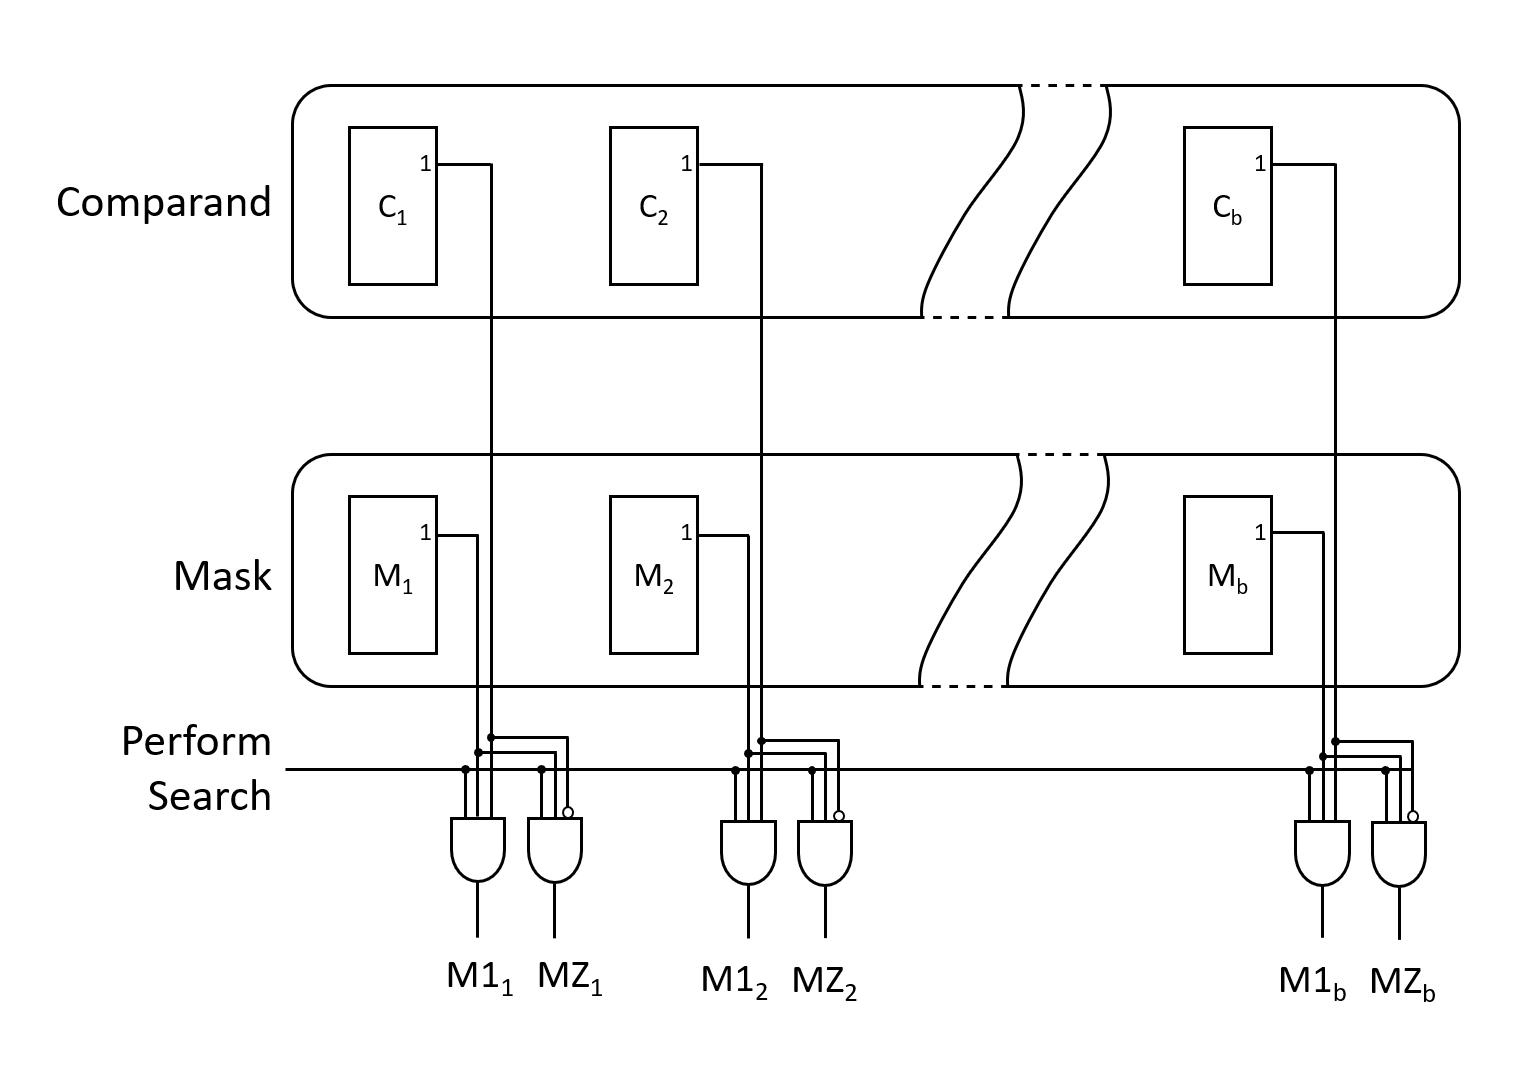
\includegraphics[height=5cm]{FPGA-CAPP_research_paper/images/search_registers.png}
  \caption{Design of the CAPP search registers}
  \label{search_circuit}
\end{figure}

The second most complex circuitry is found in the tags. Each tag is a one bit register and there is one tag associated with each memory cell. If the bit of a cell is high after a search, it means that the word in that cell matched the search criteria. In other words, after a search, the cells with high tag bits are the ones that constitute the answer set. As all the tag bits of a CAPP have to change in constant time (i.e. in parallel), match lines from the search registers go through each cell to create mismatch lines which turn irrelevant tags off whenever the search signal is set. The circuitry also includes logic for manually setting all bits high and selecting the first tag bit that is on. The design for these are given in Figure \ref{tag_registers}.

\begin{figure}
  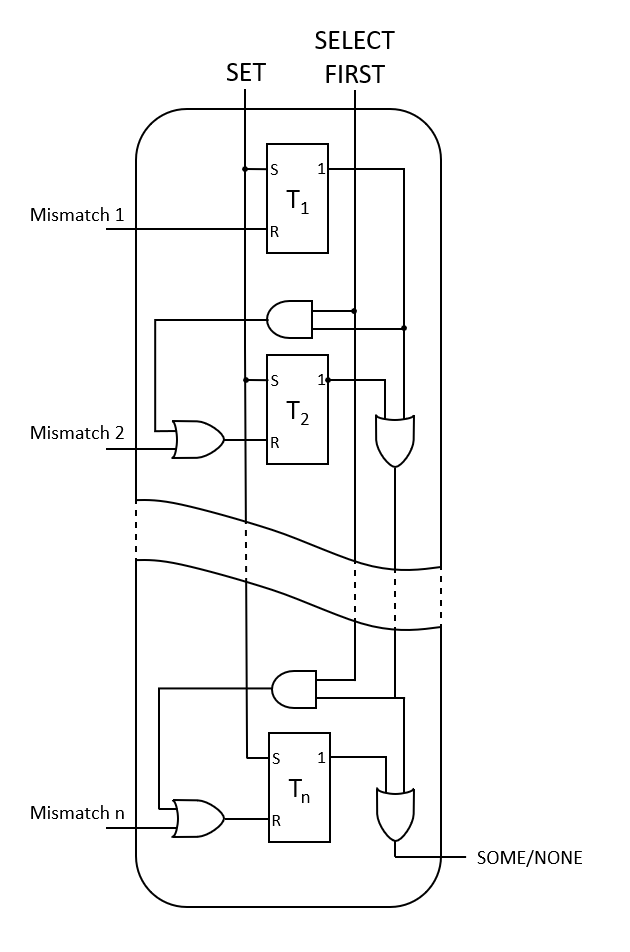
\includegraphics[height=14cm]{FPGA-CAPP_research_paper/images/tag_registers.png}
  \caption{Design of the CAPP tag registers}
  \label{tag_registers}
\end{figure}

Arguably the most complex circuitry is found in the memory cells themselves, as it encapsulates the main logic for writing, reading and searching. Each bit of each cell is surrounded by two write lines, two search lines and one read line. The n-th bits across all cells share these lines, i.e. each position has a set of lines across all the cells. The value of each bit in each cell is changed to 0 or 1 depending on which write line is set high. Conversely, depending on the two search lines and the bit value, a mismatch line that is connected to the tag bit of the cell is set high or low  (see \ref{mismatch_lines}). This allows the CAPP to search or write in parallel. The output of all the read lines is the bitwise OR of all cells that have their tag bits on as shown in Figure \ref{read_lines}. The parallel writing and reading of results is precisely what distinguishes CAPPs from the more common CAM architecture (as described in the introduction).

\begin{figure}
  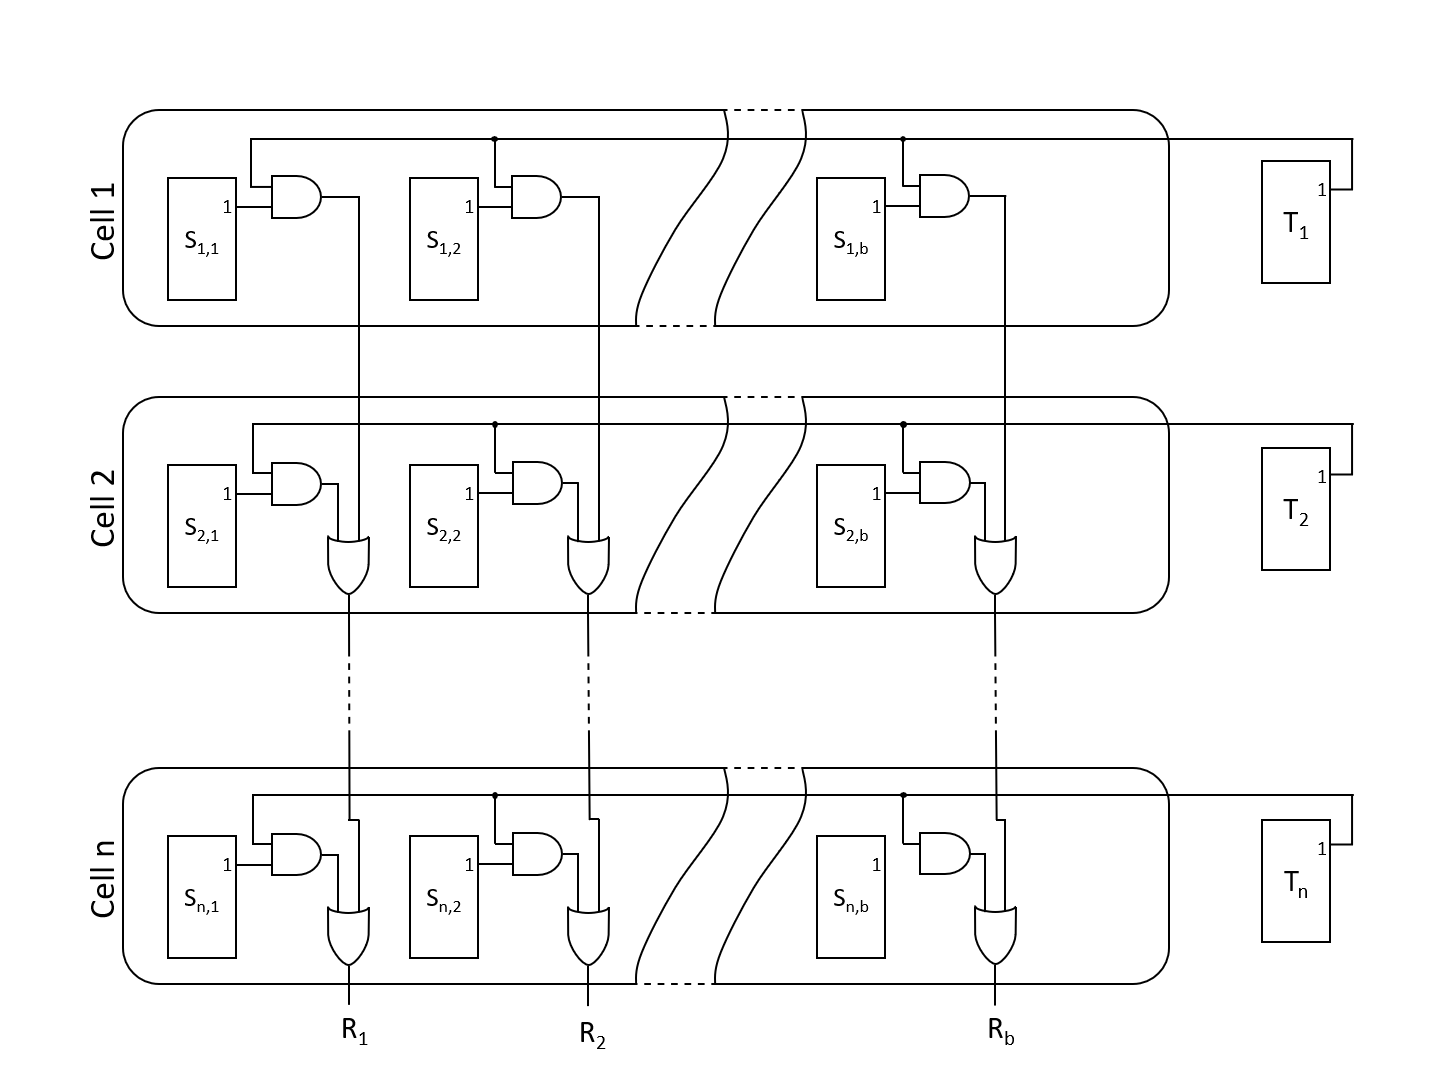
\includegraphics[height=6.5cm]{FPGA-CAPP_research_paper/images/read_lines.png}
  \caption{Design of the parallel read logic}
  \label{read_lines}
\end{figure}

\begin{figure}
  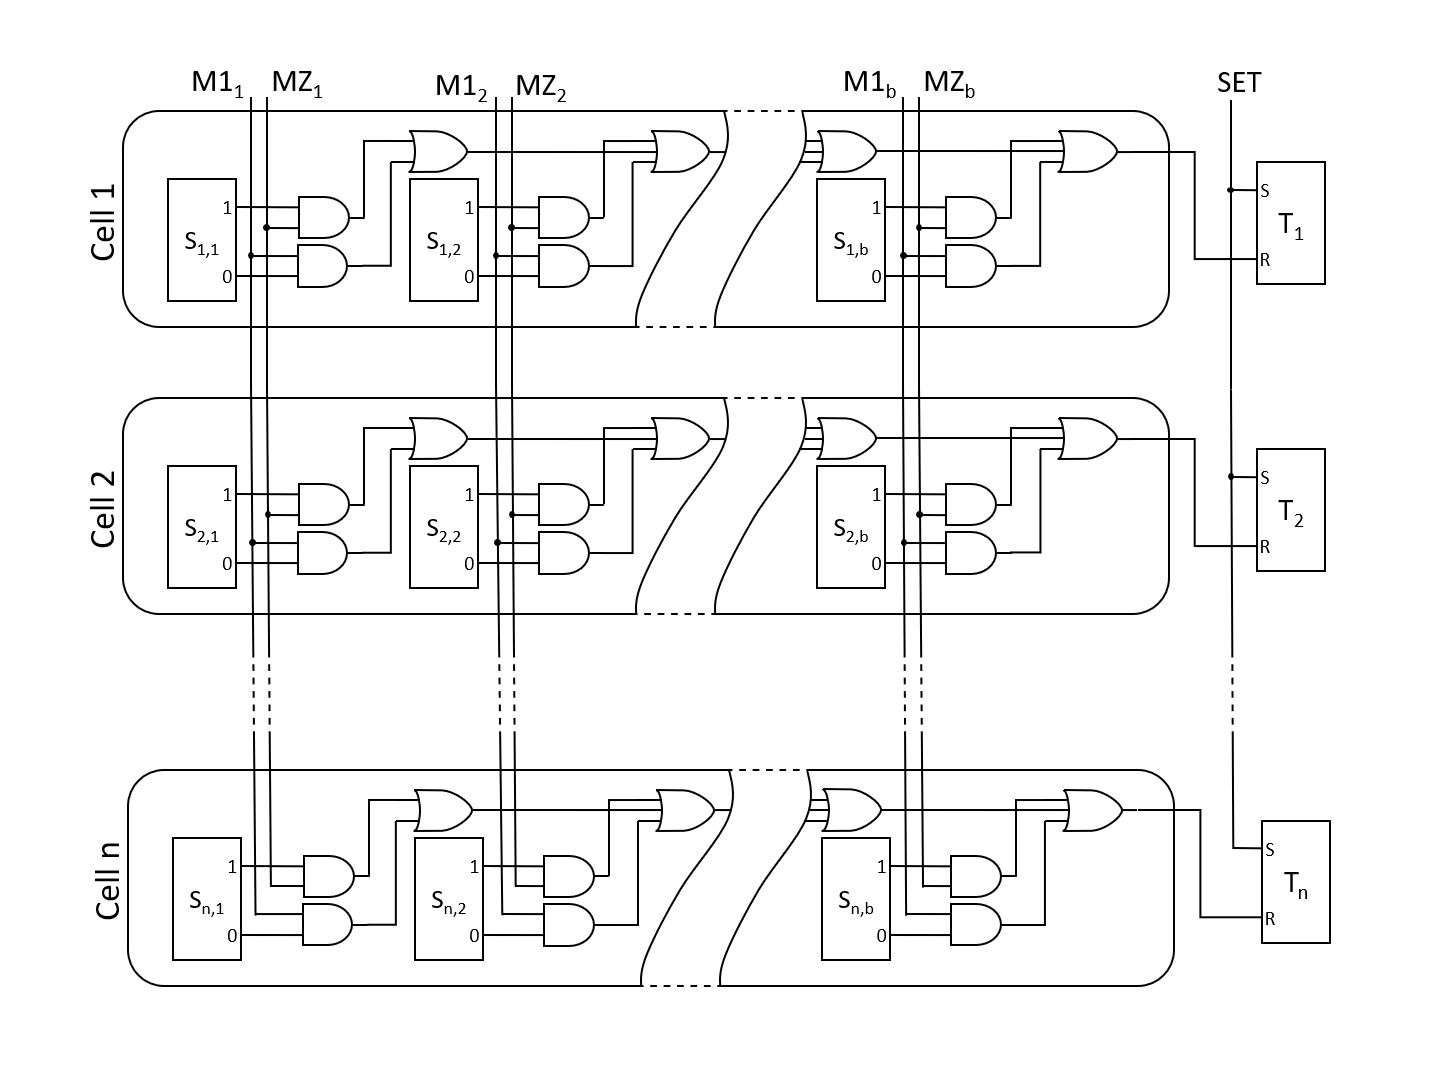
\includegraphics[height=6.5cm]{FPGA-CAPP_research_paper/images/mismatch_lines.png}
  \caption{Design of the parallel matching logic}
  \label{mismatch_lines}
\end{figure}

The design described above is identical to the introductory CAPP described in Caxton Foster's seminal book on the topic of CAPPs \cite{capp}. We implemented a direct translation to Verilog and then used nextpnr \cite{8735573} for the placing and routing of our Verilog design. The choice of nextpnr was due to its ability to take into account timing constraints which were important for the correct implementation of the Serial UART module needed to function reliably despite being connected to a CAPP module which requires potentially more than one clock cycle to execute a request communicated from the host computer. The resulting layout was synthesized and tested on the TinyFPGA-BX using a Python-based driver to communicate with the resulting USB-CAPP device.
The Finite State Machine at the core of the communication protocol between the host computer and the CAPP is described in the next section.
\section{The Finite State Machine}
The FSM is the crux of interacting with the CAPP and making it carry out complex arbitrary algorithms by exposing commands to carry out different tasks. 
It has numerous states, some of them are sending or receiving data, loading data into the CAPP, selecting first, searching, reading, setting the comparand and mask as well as writing. 
The base UART module used is from David Things' Github repository. \cite{uart} This works on a 48MHz clock cycle.
To reduce complexities and avoid additional LUTs usage, we used the same clock speed throughout the project. 

\begin{figure}
  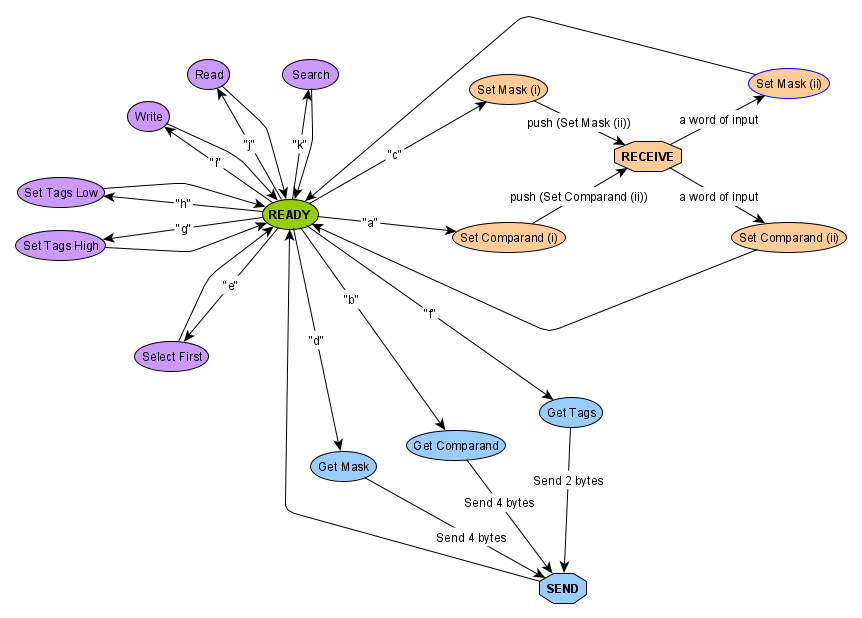
\includegraphics[height=6cm]{FPGA-CAPP research paper/images/protocol.png}
  \caption{Overview of the FSM underlying the CAPP-host protocol}
  \label{FSM_protocol}
\end{figure}

As shown in Figure \ref{FSM_protocol}, our FSM acts as a way to carry out procedural tasks while staying under the limit of 21ns by linking states together. 
Therefore, a task may trigger several states before it returns to the default state. 
For example, the algorithm for searching has several steps, it comprises of
\begin{itemize}
    \item Setting the comparand 
    \item Setting the mask 
    \item Sending the SET signal
    \item Sending the SEARCH signal 
\end{itemize}

Notice that the first two steps use several clock cycles as only one byte of data flows through the UART each clock cycle. 
This is due to its pipeline design. 

The states transitions for the SET signal is given below:
\begin{itemize}
    \item  SET 1: change SET to high, set delay to 5 clock cycles
    \item  IDLE: wait for delay, go to SET 0
    \item  SET 0: change SET to low, listen for new command
\end{itemize}
\vspace{5mm}
This is similar to the SEARCH signal:
\begin{itemize}
    \item  SEARCH 1: change SEARCH to high, set delay to 5 clock cycles
    \item  IDLE: wait for delay, go to SEARCH 0
    \item  SEARCH 0: change SEARCH to low, listen for new command
\end{itemize}
\vspace{5mm}
The tasks that involve transmitting follow a similar state transition procedure. 
Here, a state send one character to the host through the uart each clock cycle. 
Examples of these are sending comparand, tags and mask. 
The state transition diagram for sending the comparand is shown in \ref{FSM_protocol}.
The procedures for the other commands are similar in the way that different states just change the value of a register. 
The send state just transmits data from this register. 
This design decision was made to reduce the memory as well as number of combinatorial circuits. 

\begin{itemize}
    \item  GET COMPARAND: set output text to comparand
    \item  SEND: Send the next character until EOL. Listen for next command
\end{itemize}

\section{Results}
A Content Addressable Parallel Processor was successfully completed. 
The machine works in conjunction with a machine with Von Neumann architecture that is 
responsible for streaming commands to the CAPP which enacts them on the CAM. 
The commands are sent over serial using a UART module on the FPGA\\\\
As the CAPP works on the principles of a CAM, 
it can search for matching cycles in constant time, 
and write to those in constant time too. 
\\\\
We also wrote a Python library that is used to initialize the CAPP and send commands to it 
from the external Von Neumann machine. 
This makes it easy to transmit commands and read cells in the CAM. 
\section{Conclusion}
\blindtext
\section{Discussion}
\blindtext
\section*{Acknowledgment}
The authors would like to thank ... for his/her/their help and support during the process of writing this paper. \cite{webpage, FundConDep,exampleofjournalarticle,exampleofconferencepaper}
% Select the IEEEtran style
\bibliographystyle{IEEEtran}
% Include bibliography file
\bibliography{IEEEabrv,references}
\end{document}